\chapter{Επίλογος}
\label{chap8}

Στην παρούσα διπλωματική εργασία αποδείχθηκε πως η μελέτη της Μονάδας Δυναμικής Πρόβλεψης Διακλαδώσεων, όταν ορισμένα στοιχεία της αρχίζουν να υπολειτουργούν, αποτελεί πολύ βασικό αντικείμενο για την αντιμετώπιση τόσο της υποβάθμισης της απόδοσης του επεξεργαστή, όσο και της αύξησης της συνολικής κατανάλωσης που μπορεί να προκληθεί. Για πρώτη φορά παρουσιάστηκε μία τέτοια μελέτη, η οποία εντοπίζει την αιτία του προβλήματος και προτείνει κατάλληλη λύση με το ελάχιστο δυνατό κόστος.

\section{Σύνοψη και συμπεράσματα}

Παρότι τα σφάλματα της Μονάδας Δυναμικής Πρόβλεψης Διακλαδώσεων δεν έχουν ως αποτέλεσμα τη λανθασμένη εκτέλεση ενός προγράμματος, όπως αποδείχθηκε μπορούν να προκαλέσουν πολύ σημαντικό κόστος σε χρόνο και ενέργεια. Τη βασική αιτία, όπως παρουσιάστηκε στο Κεφάλαιο \ref{chap4}, αποτελούν τα σύνολα του Πίνακα Πρόβλεψης Προορισμού Διακλάδωσης των οποίων όλα τα πλαίσια είναι ελαττωματικά (πλήρως ελαττωματικά σύνολα). Η αδυναμία αποθήκευσης πληροφορίας για ένα πλήθος εντολών διακλάδωσης έχει ώς αποτέλεσμα την μείωση του ποσοστού επιτυχίας των προβλέψεων, το οποίο συνεπάγεται την εκτέλεση άσκοπων εντολών των οποίων τα αποτελέσματα τελικώς θα απορριφθούν. Τη λύση σε αυτό το πολύ σοβαρό ζήτημα έδωσε η τεχνική της λογικής μετάθεσης πλαισίων με τη χρήση ορισμένων καταχωρητών και πυλών \xor, όπως παρουσιάστηκε στο Κεφάλαιο \ref{chap5}.
\par
Όπως προέκυψε και από τη μελέτη που παρουσιάστηκε στην Ενότητα \ref{chap5_AlgorithmResults}, η προτεινόμενη τεχνική επιτυγχάνει επίλυση άνω του $50\%$ των πλήρως ελαττωματικών συνόλων, ενώ σε πολλές περιπτώσεις το ποσοστό αυτό φτάνει ακόμη και το $100\%$, με το κόστος υλοποίησης να παραμένει μικρότερο του $1\%$. Αντίστοιχα, όπως διαπιστώθηκε στο Κεφάλαιο \ref{chap6} η μείωση των πλήρως ελαττωματικών συνόλων περιόρισε την πτώση της απόδοσης εξαιτίας των σφαλμάτων από $38\%$ έως και $72\%$, ενώ την αύξηση της κατανάλωσης από $48\%$ έως και $76\%$ (Πίνακας \ref{tab:chap6_finalResults}). Επομένως, η εφαρμογή της προτεινόμενης τεχνικής σε συνδυασμό με τις μεθόδους μείωσης της τάσης λειτουργίας, συμβάλει σημαντικά στη συνολική μείωση της καταναλισκόμενης ενέργειας ενός σύστημα.

%----------------------------------------------------------%

\section{Μελλοντικές επεκτάσεις}

Σαν τελευταίο κομμάτι της παρούσας διπλωματικής εργασίας παρουσιάζεται ένα μικρό μέρος των αποτελεσμάτων της τρέχουσας έρευνας για την εφαρμογή της λογικής μετάθεσης πλαισίων στις Κρυφές Μνήμες πρώτου επιπέδου. Παρότι πληθώρα τεχνικών έχουν προταθεί για την επίλυσή τους, όπως αναφέρθηκε και στο Κεφάλαιο \ref{chap3}, η συγκεκριμένη τεχνική έχει το βασικό πλεονέκτημα του πολύ χαμηλού κόστους υλοποίησης. Στο Σχήμα \ref{fig:chap8_cache_faults} φανερώνεται η βελτίωση που θα επέφερε η εφαρμογή της μετάθεσης πλαισίων σε μία Κρυφή Μνήμη πρώτου επιπέδου μεγέθους 32\en{Kbyte}, οργάνωσης 4-τρόπων συνόλου συσχέτισης και πλαισίων των 64 ψηφιολέξεων. Τα αποτελέσματα αναφέρονται στην πιθανότητα σφάλματος $\expnum{2}$, όπου κατά μέσο όρο το $64\%$ των πλαισίων περιέχουν τουλάχιστον μία ελαττωματική κυψελίδα και συνεπώς απενεργοποιούνται.

\begin{figure}[h]
    \centering
    \fbox{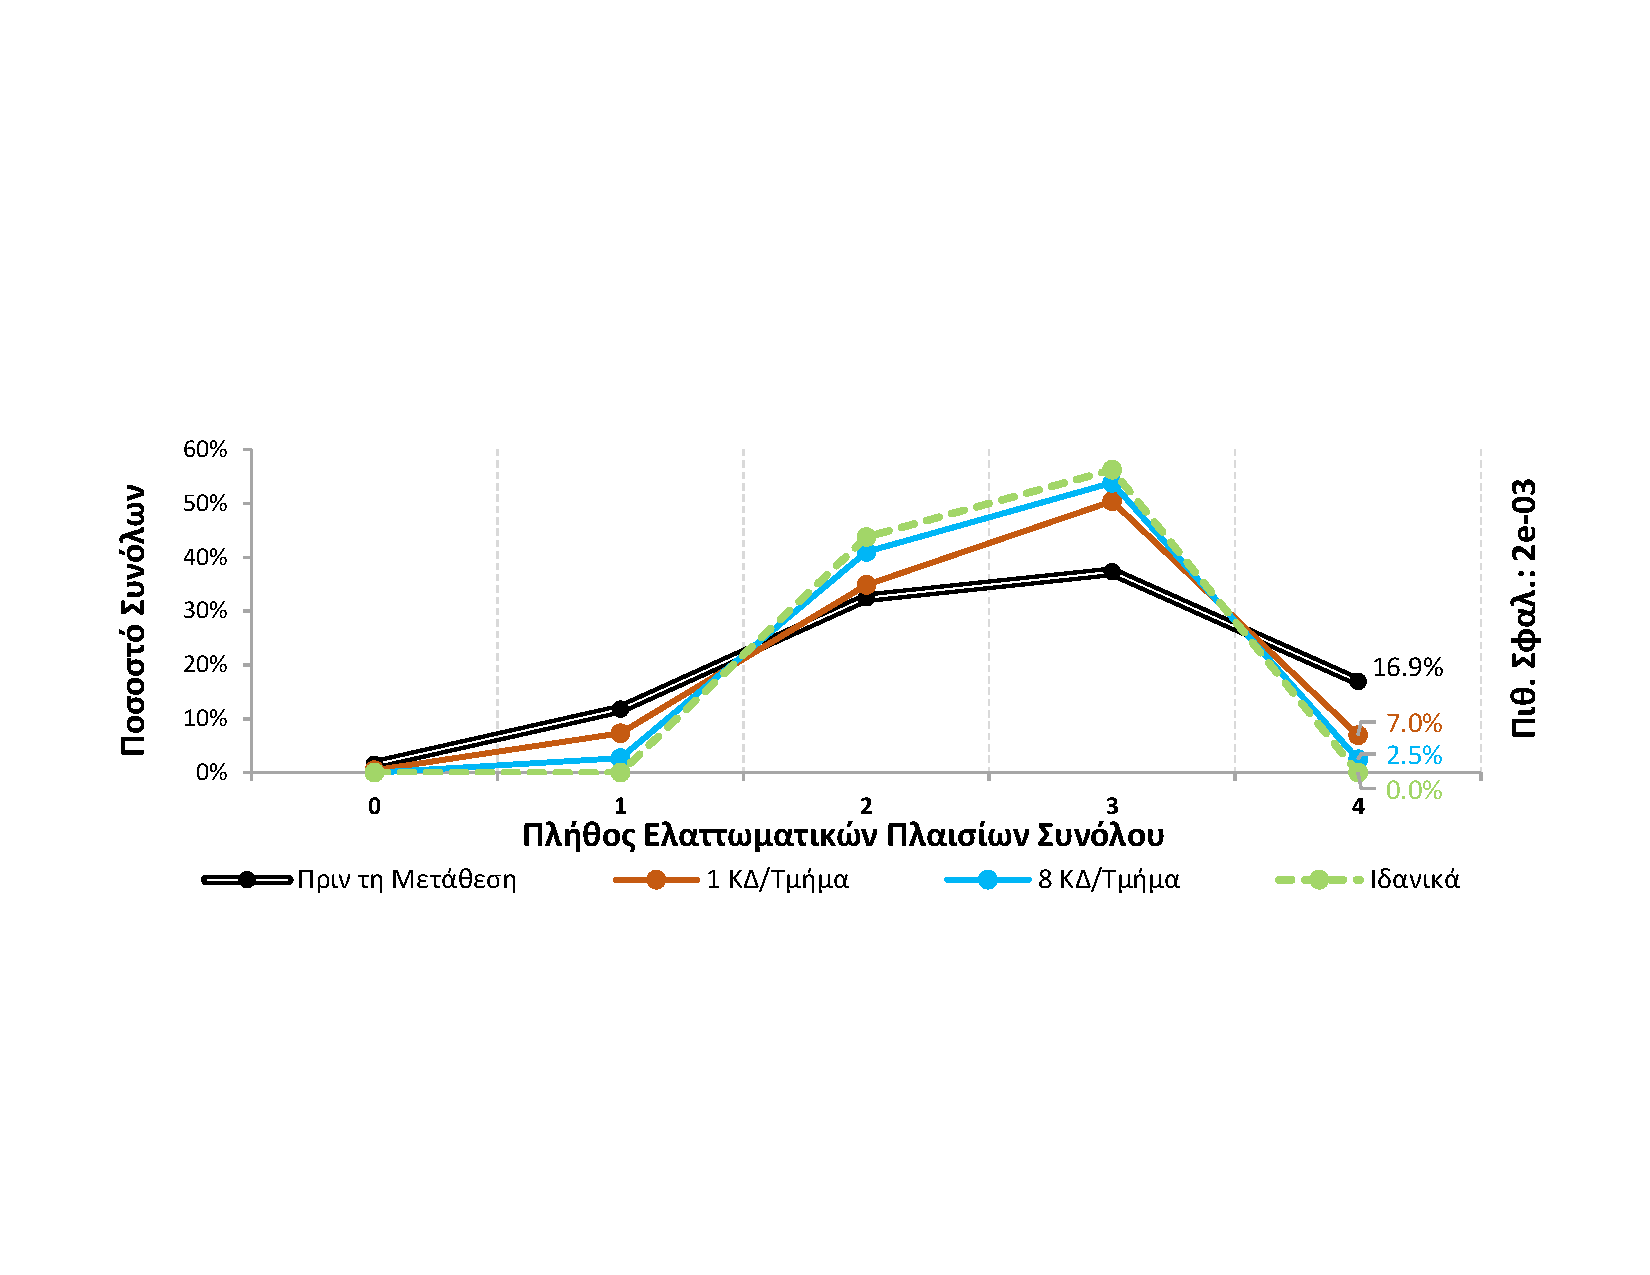
\includegraphics[width=\linewidth, trim=2cm 6.4cm 1.6cm 7.4cm, clip=true]{\resultsDIR/chap8_Cache_fault_distribution.pdf}}
    \caption{Κατανομή των σφαλμάτων στα σύνολα της Κρυφής Μνήμης πριν και μετά την εφαρμογή της μετάθεσης πλαισίων}
    \label{fig:chap8_cache_faults}
\end{figure}

Σύμφωνα με το γράφημα του Σχήματος \ref{fig:chap8_cache_faults}, όταν δεν εφαρμόζεται καμία τεχνική βελτίωσης (δείκτες μαύρου χρώματος - διπλή γραμμή) το $16.9\%$ των συνόλων περιέχουν 4 ελαττωματικά πλαίσια (πλήρως ελαττωματικά σύνολα) με αποτέλεσμα να μην είναι δυνατή η αποθήκευση πληροφορίας σε αυτά, αυξάνοντας έτσι το ποσοστό αστοχίας της μνήμης. Με το ποσοστό των ελαττωματικών πλαισίων να αγγίζει το $64\%$, στην ιδανική περίπτωση (δείκτες πράσινου χρώματος - διακεκομμένη γραμμή) θα μπορούσε να πραγματοποιηθεί τέτοια κατανομή ώστε στο $56\%$ των συνόλων τα 3 από τα 4 πλαίσια να είναι ελαττωματικά, ενώ στο υπόλοιπο $44\%$ τα 2 από τα 4. Με τον τρόπο αυτό όλα τα σύνολα θα είχαν τουλάχιστον ένα διαθέσιμο πλαίσιο. Όπως φανερώνεται και από το γράφημα, εάν χρησιμοποιηθεί ένας Καταχωρητής Διαμόρφωσης ανά τμήμα (δείκτες πορτοκαλί χρώματος) τα πλήρως ελαττωματικά σύνολα μειώνονται σε $7\%$, ενώ με τη χρήση 8 καταχωρητών ανά τμήμα (δείκτες γαλάζιου χρώματος) το ποσοστό αυτό μειώνεται σε μόλις $2.5\%$. Επομένως, η εφαρμογή της τεχνικής στην Κρυφή Μνήμη πρώτου επιπέδου θα έδινε τη δυνατότητα επιτυχίας στο $97.5\%$ των διευθύνσεων προσπέλασης από $83.1\%$ που είναι αρχικά. Η εφαρμογή της συγκεκριμένης τεχνικής αναμένεται να αποδειχθεί πολύτιμη στον τομέα της ανοχής σφαλμάτων των Κρυφών Μνημών, εξαιτίας του πολύ μικρού κόστους που επιφέρει σε συνδυασμό με την υψηλή αποδοτικότητα και προσαρμοστικότητά της.

%----------------------------------------------------------%
